\begin{pastexam}[label={px:gk3-105-ds-01}]{高考三級資訊處理 105 年 第一題}
（申論；20 分）

假設一個無向圖（undirected graph）的邊（edges）如下：
\begin{center}
S, T \quad S, Z \quad T, Y \quad T, Z \quad V, Y \quad V, Z \quad Y, Z
\end{center}
\begin{itemize}[leftmargin=2.2em]
\item[㈠] 使用堆疊（stack），從 S 開始，進行深度優先走訪（depth-first traversal），請寫出走訪結果。（10 分）
\item[㈡] 使用佇列（queue），從 S 開始，進行廣度優先走訪（breadth-first traversal），請寫出走訪結果。（10 分）
\end{itemize}
\end{pastexam}

\begin{pastsoln}
答案：㈠ $S, T, Y, V, Z$；㈡ $S, T, Z, Y, V$。

題目沒有規定同時有好幾個相鄰頂點時先走哪一個，這裡照字母順序先處理小的（教科書的慣例，答案卷上
要寫明這個約定）。 先把圖和鄰接串列寫出來（每個串列依字母排序）：
\begin{center}
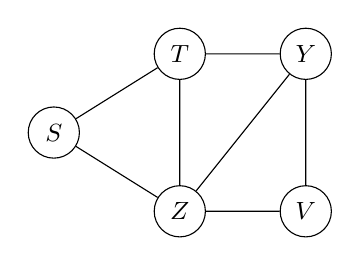
\begin{tikzpicture}[v/.style={circle,draw,minimum size=6.5mm,inner sep=0pt,font=\small}]
\node[v] (S) at (0,0) {$S$};
\node[v] (T) at (1.6,1) {$T$};
\node[v] (Z) at (1.6,-1) {$Z$};
\node[v] (Y) at (3.2,1) {$Y$};
\node[v] (V) at (3.2,-1) {$V$};
\draw (S)--(T) (S)--(Z) (T)--(Y) (T)--(Z) (V)--(Y) (V)--(Z) (Y)--(Z);
\end{tikzpicture}
\qquad
\begin{tabular}[b]{ll}
\toprule
頂點 & 相鄰頂點 \\
\midrule
$S$ & $T, Z$ \\
$T$ & $S, Y, Z$ \\
$V$ & $Y, Z$ \\
$Y$ & $T, V, Z$ \\
$Z$ & $S, T, V, Y$ \\
\bottomrule
\end{tabular}
\end{center}

\textbf{㈠ 用堆疊的深度優先走訪}（資結書第~21.4~節、虛擬碼~21.4）。 做法：pop 出一個頂點，若還沒
走過就走訪它，再把它還沒走過的相鄰頂點\textbf{反著字母順序} push 進去，這樣字母小的在堆疊頂端，
下一個先被 pop。 堆疊由左寫到右，右端是頂端：
\begin{center}
\begin{tabular}{llll}
\toprule
步驟 & pop & 走訪 & push 之後的堆疊 \\
\midrule
0 & & & $S$ \\
1 & $S$ & $S$ & $Z, T$ \\
2 & $T$ & $T$ & $Z, Z, Y$ \\
3 & $Y$ & $Y$ & $Z, Z, Z, V$ \\
4 & $V$ & $V$ & $Z, Z, Z, Z$ \\
5 & $Z$ & $Z$ & $Z, Z, Z$ \\
6--8 & $Z$ & （走過了，丟掉） & 空 \\
\bottomrule
\end{tabular}
\end{center}
走訪順序 $S, T, Y, V, Z$。 和遞迴版的 DFS（每次往字母最小、還沒走過的鄰居走）結果相同：
$S \to T \to Y \to V \to Z$，一路走到底，沒有回頭分岔。

\textbf{㈡ 用佇列的廣度優先走訪}（資結書第~21.3~節、虛擬碼~21.1）。 頂點放進佇列時就標記，避免重複
放入；佇列左端是前端：
\begin{center}
\begin{tabular}{llll}
\toprule
步驟 & 取出走訪 & 放入（新發現的鄰居） & 佇列 \\
\midrule
0 & & $S$ & $S$ \\
1 & $S$ & $T, Z$ & $T, Z$ \\
2 & $T$ & $Y$（$S$、$Z$ 已標記） & $Z, Y$ \\
3 & $Z$ & $V$（$S, T, Y$ 已標記） & $Y, V$ \\
4 & $Y$ & 無 & $V$ \\
5 & $V$ & 無 & 空 \\
\bottomrule
\end{tabular}
\end{center}
走訪順序 $S, T, Z, Y, V$。 依距離分層：距離 $0$ 是 $S$，距離 $1$ 是 $T, Z$，距離 $2$ 是 $Y, V$。
\end{pastsoln}
